\chapter{Methodology}  \label{ch:methodology}

\subsection{Machine learning techniques}


\begin{table}[h]
\centering
 \begin{tabular}{l l} 
 \hline
 SYMBOL & DESCRIPTION \\ 
 \hline
 $K$ & Number of Topics \\  
 $V$ & Number of words in the vocabulary \\
 $M$ & Number of documents \\
 $N$ & Number of words in the document \\
 $N_{d=1..M}$ & Number of words in document d\\
 $\alpha$ & ?? \\
 $\alpha_{k=1...K}$ & Hyperparameter for dirichlet prior distribution of topic $k$ \\
 $\beta$ & collection of all $\beta$ \\
 $\beta_{w=1...V}$ & Hyperparameter for dirichlet prior distribution of a word $w$ in a topic \\
 $\varphi_{k=1...K}$ & Distribution of words in topic $k$ \\
 $\varphi_{k=1...K, w=1...V}$ & Probability of  word $w$ in topic $k$  \\
 $\theta{d=1...M}$ & Distribution of topics in document $d$  \\
 $\theta{d=1...M, k=1...K}$ & Probability of  topic $k$ in document $d$ \\
 $z_{d=1...M}, w=1...N_d$ & Assigned topic of word $w$ in document $d$\\
 $Z$ & Topic of all words in documents \\
 $w_{d=1...M, w=...N_d}$ & Assigned word w in document d \\ 
 $W$ & Words in all documents \\ 

 

 
 \hline
 \end{tabular}
\caption{Notation of used in paper}
\label{tab:table1}
\end{table}

\section{Topic Modelling}
Topic models are algorithms used to find themes in mostly large unstructured collections of documents \cite{Blei2010ProbabilisticModels}. Where humans have a hard time to find a structure, topic modelling uses statistical methods for analyzing words for topic discovery. This makes it possible to compare topics with each other, find similar documents without necessarily having any prior knowledge of your collection. 


\section{Latent dirichlet allocation}
In natural language processing \textit{Latent dirichlet allocation} (LDA) is an unsupervised machine learning technique introduced in 2003 for Topic modelling \cite{Blei2003LatentAllocation}. A general assignment of notations for LDA can be seen in table \ref{tab:table1}

LDA makes use of a generative probabilistic model of a collection of documents \textbf{M} to discover latent topics, Fig \ref{fig:LDA} represents this model. This method assumes that each document \textbf{N} in the corpus contains a mixture of latent topics. These topics are a mixture of words \textbf{W} assigned to a topic from a fixed vocabulary \textbf{V}. \textbf{Z} Notates the assignment of words to a topic. The distribution of words $\theta$ for each topic is dependent on the sensitivity of $\alpha$. A low $\alpha$ means that the topic contains a distinct (sparse) representation of words and a high $\alpha$ means that topics have more generative words. The probability distribution of topics in documents $\varphi$ are depended on the sensitivity of $\beta$. A low $\beta$ means that documents contain distinct topics and a high $\beta$ is a mixture of multiple topics in a document. The number of topics \textbf{K} are predefined in LDA. 

\begin{figure}
    \centering
    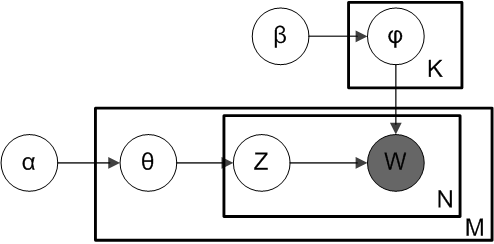
\includegraphics[h]{methodology/Smoothed_LDA.png}
    \caption{A smoothed LDA plate notation}
    \label{fig:LDA}
\end{figure}

The LDA algorithm is defined in 3 steps:
\begin{enumerate}
    \item For each document, pick a topic from its distribution over topics.
    \item Sample a word from the distribution over the words associated with the chosen topic. 
    \item  The process is repeated for all the words in the document.
\end{enumerate}

This process can also be described as the assignment of a topic proportion $\varphi$ to a document. Following this assignment each word W from the document gets an assignment Z of a random topic K from the assigned topics $\varphi$. These steps are repeated for the amount of W in document N.

\subsection{$\alpha$ and $\beta$ hyperparameters} 
In Bayesian statistics, a hyperparameter is a parameter of a prior distribution; the term is used to distinguish them from parameters of the model for the underlying system under analysis. 
$\alpha$ is the parameter of the Dirichlet prior on the per-document topic distributions.
$\beta$ is the parameter of the Dirichlet prior on the per-topic word distribution.

\subsection{$\theta$, $\varphi$, Z parameters}


\section{Online Latent dirichlet allocation}
Online \cite{Hoffman2010OnlineAllocation}